\documentclass[tikz,border=6pt]{standalone}
\usepackage{times}
\usepackage{amsmath,amssymb}
\usetikzlibrary{positioning,fit,backgrounds,calc,arrows.meta,shapes.geometric}
\begin{document}
\small
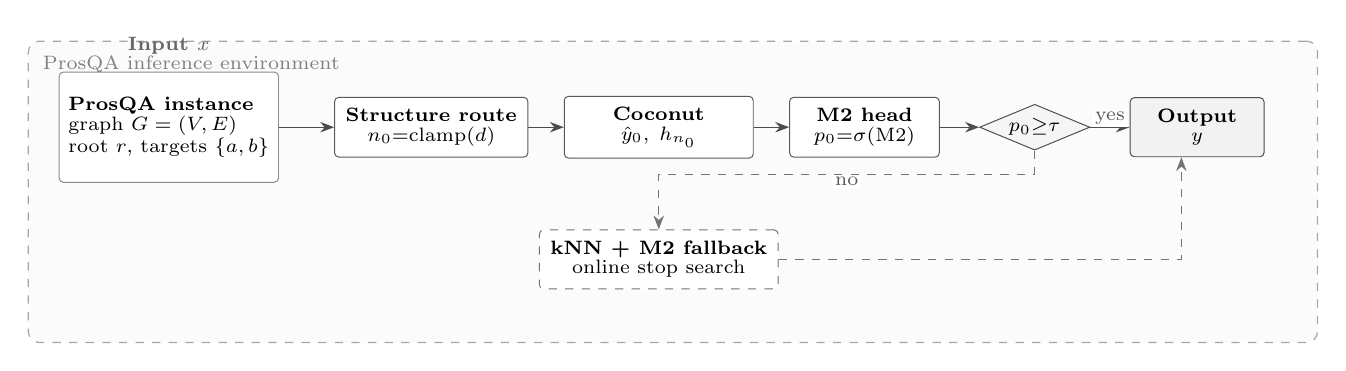
\begin{tikzpicture}[
  font=\small,
  >=Stealth,
  module/.style={
    rectangle, draw=black!65, line width=0.35pt,
    fill=white, rounded corners=1.5pt,
    minimum height=7.5mm, inner sep=4pt, align=center
  },
  smallmod/.style={
    module, minimum width=19mm, font=\scriptsize
  },
  widemod/.style={
    module, minimum width=24mm, font=\scriptsize
  },
  agentpad/.style={
    rectangle, draw=black!40, line width=0.35pt,
    fill=black!3, rounded corners=3pt, inner sep=7pt
  },
  envpad/.style={
    rectangle, draw=black!35, line width=0.45pt, dashed,
    fill=black!1.5, rounded corners=4pt, inner sep=10pt
  },
  inst/.style={
    rectangle, draw=black!45, line width=0.35pt,
    fill=white, rounded corners=1.5pt,
    minimum width=21mm, minimum height=14mm,
    align=left, font=\scriptsize
  },
  gate/.style={
    diamond, draw=black!70, line width=0.35pt,
    fill=black!4, aspect=2.1, inner sep=0.5pt,
    minimum width=14mm, font=\scriptsize, align=center
  },
  outbox/.style={
    module, minimum width=17mm, draw=black!70,
    fill=black!5, font=\scriptsize\bfseries
  },
  fb/.style={
    module, minimum width=28mm, draw=black!55, dashed,
    fill=white, font=\scriptsize
  },
  arr/.style={->, line width=0.45pt, draw=black!70},
  dasharr/.style={->, line width=0.45pt, draw=black!55, dashed},
  edgelbl/.style={font=\scriptsize, fill=white, inner sep=1pt, text=black!65}
]

\node[inst] (inst) {%
  \textbf{ProsQA instance}\\[-1pt]
  graph $G=(V,E)$\\
  root $r$, targets $\{a,b\}$%
};

\node[widemod, right=7mm of inst] (route) {%
  \textbf{Structure route}\\[-1pt]
  $n_0{=}\mathrm{clamp}(d)$%
};
\node[widemod, right=4.5mm of route] (coco) {%
  \textbf{Coconut}\\[-1pt]
  $\hat y_0,\; h_{n_0}$%
};
\node[smallmod, right=4.5mm of coco] (m2) {%
  \textbf{M2 head}\\[-1pt]
  $p_0{=}\sigma(\mathrm{M2})$%
};
\node[gate, right=5mm of m2] (gate) {$p_0{\ge}\tau$};
\node[outbox, right=5mm of gate] (out) {%
  \textbf{Output}\\[-1pt]
  $y$%
};

\node[fb, below=9mm of coco] (fb) {%
  \textbf{kNN + M2 fallback}\\[-1pt]
  online stop search%
};

\begin{scope}[on background layer]
  \node[agentpad, fit=(route) (coco) (m2) (gate) (fb) (out), inner sep=8pt] (agentbox) {};
  \node[anchor=north west, font=\scriptsize\bfseries, text=black!55]
    at ([xshift=2pt,yshift=-2pt]agentbox.north west) {confidence\_fallback agent};
\end{scope}

\begin{scope}[on background layer]
  \node[envpad, fit=(inst) (agentbox), inner sep=11pt] (envbox) {};
  \node[anchor=north west, font=\scriptsize, text=black!50]
    at ([xshift=2pt,yshift=-2pt]envbox.north west) {ProsQA inference environment};
\end{scope}

\draw[arr] (inst) -- (route);
\draw[arr] (route) -- (coco);
\draw[arr] (coco) -- (m2);
\draw[arr] (m2) -- (gate);
\draw[arr] (gate) -- node[edgelbl, above] {yes} (out);

\draw[dasharr] (gate.south) -- ++(0,-3mm) -| node[edgelbl, pos=0.25, below] {no} (fb.north);
\draw[dasharr] (fb.east) -| ([xshift=-2mm]out.south);

\node[font=\scriptsize\bfseries, text=black!60, above=1mm of inst]
  {Input $x$};

\end{tikzpicture}
\end{document}
